\documentclass[a4paper,10pt]{article}

% Hier die Nummer des Blatts und Autoren angeben.
\newcommand{\blatt}{1}
\newcommand{\autor}{Till Schander (6682565)}

\usepackage{hci}

\begin{document}
% Seitenkopf mit Informationen
\kopf
\renewcommand{\figurename}{Abbildung}

\aufgabe{1}
\begin{enumerate}

\item Anforderungen:
\begin{itemize}
	\item Standort auf Karte anzeigen
	\item Landmarken speichern
	\item Offline nutzbar
	\item Kälte-resistent
	\item Wasser-resistent
	\item Energiesparend
	\item Mit Handschuhen bedienbar
	\item Geringes Gewicht
\end{itemize}
	
\item Zeichnung:
\begin{figure}[ht]
\centering 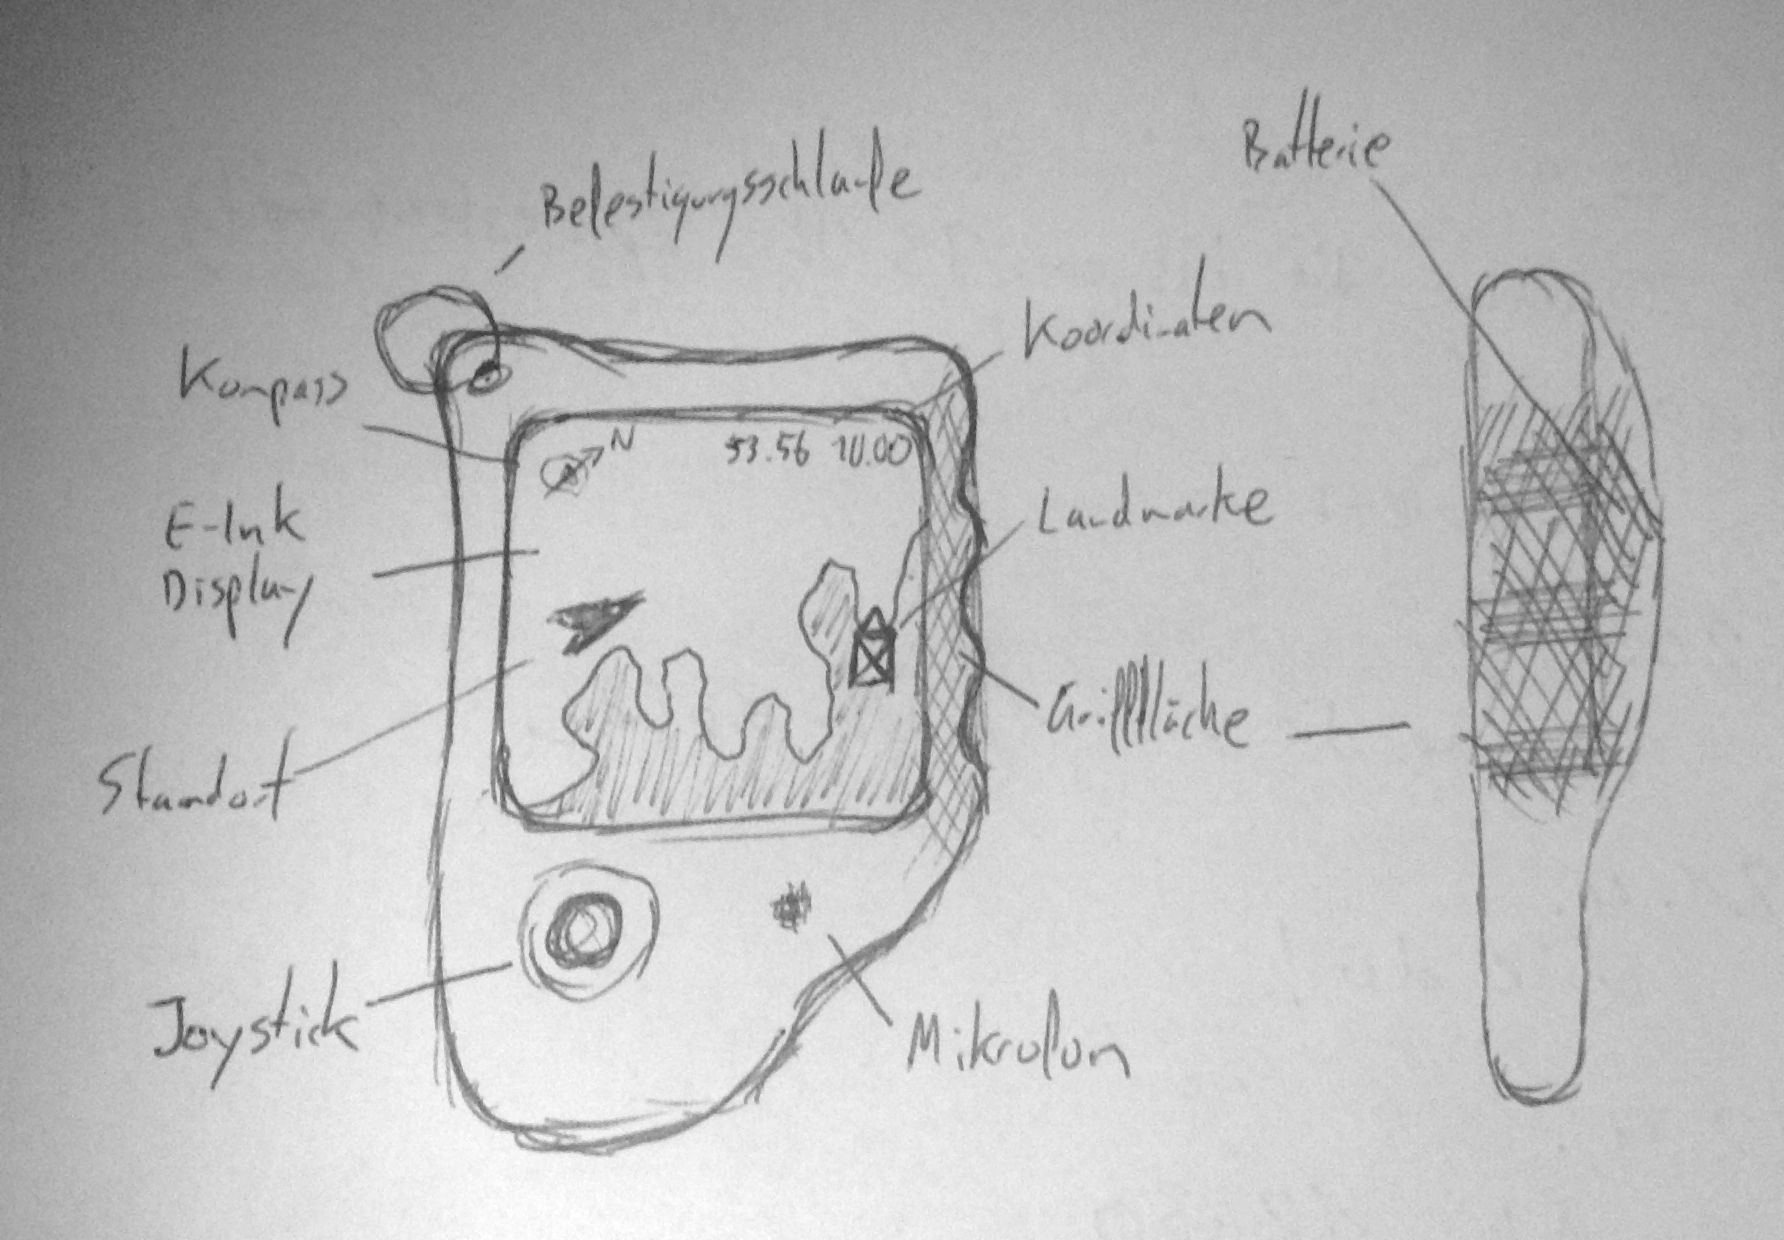
\includegraphics[width=0.7\textwidth]{icg1.jpg}
\caption{Skizze des Produkts}
\end{figure}

\item Beschreibung:\newline
Das Navigationsgerät für die Inuit-Indianer muss speziellen Anforderungen genügen, die nicht für normale Navigationsgeräte gelten. Zu erst sollte es natürlich den Aktuellen Standort auf einer Karte anzeigen. Hierbei ist zu beachten, dass Mobilfunkempfang in Grönland vermutlich sehr eingeschränkt ist. Karten sollten daher offline verfügbar sein. Der aktuelle Standort kann via GPS empfangen werden. Zusätzlich kann ein eingebauter Kompass die Navigation erleichtern. Da sich das Gelände und die See durch Eis bzw. Schnee stark verändern kann, ist es nützlich aktuelle Landmarken auf dem Gerät zu speichern, die nicht auf der Karte eingezeichnet sind. Die Bedienung des Geräts muss aufgrund der kalten Temperaturen auch mit Handschuhen noch möglich sein. Daher wird auf filigrane Eingabemethoden verzichtet und ein Joystick und Sprachsteuerung eingebaut. Raue Griffflächen geben mehr Halt. Natürlich sollte das Gerät an sich auch den niedrigen Temperaturen standhalten. Zusätzlich sollte es Wasser-resistent sein, da die Inuit größere Strecken im Kajak zurücklegen. Für solche größeren Strecken sollte es auch sehr leicht sein, damit keine zusätzliche Gewichtsbelastung auftritt. Da es in Grönland kaum Steckdosen gibt muss das Gerät sehr energiesparend sein. Hier hilft das E-Ink Display und auswechselbare Batterien.

\end{enumerate}

\end{document}
